%!TEX root = ../template.tex
%%%%%%%%%%%%%%%%%%%%%%%%%%%%%%%%%%%%%%%%%%%%%%%%%%%%%%%%%%%%%%%%%%%%
%% chapter2.tex
%% NOVA thesis document file
%%
%% Chapter with the template manual
%%%%%%%%%%%%%%%%%%%%%%%%%%%%%%%%%%%%%%%%%%%%%%%%%%%%%%%%%%%%%%%%%%%%

\typeout{NT FILE chapter2.tex}%

\chapter{Related Work}
\label{cha:related_work}
% TODO: add some introduction to this chapter

\section{Gossip Protocol}
\label{sec:gossip_protocol}

\subsection{History and Overview}
\label{subsec:gossip_history_overview}
The gossip protocol, also known as epidemic protocol, as the name indicates, was created
based on how gossips are propagated in social groups. In a gossip protocol, nodes in a
network send the information, randomly, to other nodes in the same network, similar to how a
gossip is spread between members in a social group \cite{Leitao2007}.

The gossip protocol is known as a highly scalable and resilient approach to implement
reliable broadcast. This protocol is based on every participant propagating their messages
collaboratively with all the members of their group.

This process starts when a node desires to propagate some piece of information to the
other members of his network. This node will send his message to \textit{t} nodes,
chosen randomly, (\textit{t} being a parameter called \textit{fanout}, which is better
explaned in the subsection \ref{subsec:gossip_parameters}). When the receiving nodes obtain the
message for the first time, they will do the same as the previous node had done and
resend the message to \textit{t}, randomly chosen nodes. If a node receives the same
message twice, it will discard it. When this happens, which may occour quite often,
since the nodes are unaware of which nodes have already received a message, there is
redundancy.

However, since neither node knows who has received each message and who has sent a
message to whom, each node will have to keep a log of all messages that he has already
received.

% TODO: types of gossip, rumor mongering, etc (see birman2007)
% TODO: partial view
% TODO: (Talk about the problems it helped solve)


\subsection{Parameters}
\label{subsec:gossip_parameters}
% TODO
\begin{description}
    \item[Fanout:]
    \item[Maximum Rounds:]
\end{description}


\subsection{Strategies}
\label{subsec:gossip_strategies}
The Gossip Protocol may be executed following different approaches \cite{Karp2000}:
\begin{description}
    \item[Eager push approach:] As soon as a node receive a message for the first time,
        it sends it to \textit{t} randomly selected nodes. This approach consumes a great
        amount of bandwidth, considering it leads to multiple copies of the same messages
        are delivered to each target node.
    \item[Pull approach:] Regularly, nodes inquire each other on new messages they've
        recently receive. If they adquire information about a message they haven't receive
        yet, they will request it expecifically from that node. This approach leads to higher
        values of latency, derivated from the extra round trip needed to obtain the messages.
    \item[Lazy push approach:] When a node receive a message for the first time, it will only
        broadcast to its neighbours a small fraction of the message, a identifier, per example
        a hash of the message. If the neighbour never receive the given identifier it will request
        the rest of the message. As in the pull approach, there will be a higher value of latency.
\end{description}

Besides the diferences in latency and bandwidth previously mentioned, there is another important
distinction between the eager push approach and the pull and lazy push approaches.
Considering that the eager push approach sends the entirety of each message immediatly after
receiving it, the nodes do not need to manitain a copy of these messages, contrarly to the
other two approaches that may need to resend these messages later. This leads to a higher
memory requirement for these approaches \cite{Leitao2012}.

By combining the approaches studied above, we can get better results, obtaining a better
latency/bandwidth tradeof. This are two of the studied combined approaches \cite{Carvalho2007}:
\begin{description}
    \item[Eager push and pull approach:] This method is divided between two distinct phases.
        The first phase consists on using the eager push approach to disseminate messages
        straightly to the nodes in the network. The second phase uses the pull approach to
        recover the lacunas that might have occoured during the first phase of this method.
        This approach reduces the amount of redundancy in comparinse with the eager push
        approach, without decreasing its performance. It will, however, endure a higher level
        of latency due to the pull phase.
    \item[Eager push and lazy push approach:] It is used the eager push approach to a subset of
        nodes. Then it uses the lazy push approach on the remaing subset of nodes to recover
        the lacunas and guarantee the reliable of the method.
\end{description}


\subsection{Tree-based Approaches}
\label{subsec:gossip_tree_based_approaches}
Tree-based broadcasting methods have a small message complexity, however, they are not
particularly resilient to faults. On the other hand, gossip protocols, as mentioned earlier
in subsection \ref{subsec:gossip_history_overview}, are known for their resilience, but have a
high message complexity \cite{Leitao2007Tree}.

In order to obtain a small message complexity and high reliability, it was considered
combining both these methods.

With this protocol we obtain the nodes organized in a tree structure formate, where each node
knows to whom foward its messages. To achieve this structure we have many approaches,
per example the PlumTree protocols:
\begin{description}
    \item[PlumTree protocol] This protocol uses eager push and lazy push gossip, previously
        explaned in the subsection \ref{subsec:gossip_strategies}. It separates the nodes in the
        network in two subsets of randomly selected nodes. The first subset of nodes uses the
        eager push protocol to disseminate the messages, while the other uses the lazy push
        protocol. The links that the eager push method uses to propagate the messages are
        chosen to create a randomized broadcast network using a tree-based structure. While
        the links used during the lazy push gossip are used to ensure the reliability of the
        method when nodes fail and potencially heal the broadcast tree when needed \cite{Leitao2007Tree}.
\end{description}

Additionally, in opposition to other gossip protocols, with tree-based gossip the connections
first made by the eager push propagating will remain until it is detected a failure. This will
allow us to use TCP connections, which will provide extra reliability and failure detection.


\subsection{Examples}
\label{subsec:gossip_examples}
Throughout many years there have been proposed numerous gossip-based protocols. During this
section we will discuss some of them:
\begin{description}
    \item[\Gls{Scamp}:] Contrarly to many other gossip-based protocols, with scamp it is
        proposed that the individual nodes have a randomized partial view of the global
        members in the network, leading to a fully descentralized system. This is quite an
        important advantage for large scale groups, since it requires a significant amount
        of memory and generates a lot of network traffic to maintain the system's overall
        consistency in extensive groups. Additionally, the scalable membership protocol is
        also compelling for its natural increase and reorganization of the partial view of
        the system when new nodes are added to the network. Having this partial view around
        \textit{log n} nodes (being \textit{n} the number of overall nodes in the network)
        \cite{Ganesh2001}.
    \item[\Gls{NeEM}:] One of the biggest problems in most gossip-based protocols is when the
        network gets congested and, subsequentially, the messages get lost. NeEM uses \Gls{TCP}
        to disseminate the messages and resolve this problem, with the usage of its ineherant
        flow and congestion control mechanisms. In order to maintain the protocol's stability,
        NeEM uses a buffer management technique that utilizes different approaches to discard
        messages on overflow. It also includes the knowledge about the messages' types in order
        to ensure that the buffer retains enough space and bandwidth is used to better fit each
        request \cite{Pereira2003}.
    \item[\Gls{CREW}:] Crew is a gossip-based protocol designed to minimize the messages
        dissemination speed. This is acquired by maintaining in cache the information about
        the already established connections, which will reduce the latency of reopening a
        TCP connection \cite{Deshpande2006}.
        % TODO: scribe and potencially MON
    \item[Scribe:] Scribe is a large scale and fully descentralized
\end{description}


\subsection{Gossip Limitations}
\label{subsec:gossip_limitations}
Throughout this section it has been vastly mentioned the advantages provided by the gossip
protocol. Mainly, it was refered the resilience and scalability offered by this method.
However, as any other protocol, it has its limitations. A few of this are \cite{Birman2007}:
\begin{enumerate}
    \item Fixed maximum message size - the gossip protocol has a fixed maximum message size
          which may lead to problems. Per exemple, if we desire to propagate a message with a
          greater size than this fixed maximum message size, we will have to divide the message
          into multiple messages. When this happens, some of these messages may be lost, since
          each node can only gossip a certain amount of information per round, which will
          increase the number of rounds to deliver a single message.
    \item Slow rate - the rate of messages exchange in a gossip protocol is typically quite
          slow, which can cause some complications when handling sudden events. This situation
          might be surpassed by reducing the periodicity of messages exchanges, however, this
          often leads to yet another problem, the increasing of overheads.
    \item Malicious behaviours and correlated loss patterns - another gossip protocol's limitation
          is when the nodes behave in a malicious form, intentionally, with disseminating of
          false information or when nodes malfunction, or unitentionally, when multiple nodes
          fail or become unavailable at the same time.
\end{enumerate}


\subsection{Discution}
\label{subsec:gossip_discution}
Throughout this section \ref{sec:gossip_protocol} it has been explained the basis of the
gossip protocol, its strategies, tree-based approaches, particularly the PlumTree, it was
also mentioned some interesting examples of gossip-based methods and finally its limitations.

This protocol is crutial for the development of my dissertation, since it is highly scalable
and reliable, which is fundamental for dealing with the messages exchanges between all cows.
Every cow will have to be constantly informed on the fence location, since it can potencially
change. Using the gossip protocol to disseminate this information seems benefic.

The PlumTree approach is quite interesting for my dilema considering that every herd has a
leader that commands all the other cows in the group. With a tree-based strategy this cow
appears to be an obvious choice to be the root and send the information throughout the
entire herd.


\section{Wireless Sensor Networks}
\label{sec:wireless_sensor_networks}

\subsection{Definition}
\label{subsec:wsn_definition}
\Gls{WSN} is an innovative technology with immeasurable applications ranging from remote
environmental monotorization to target tracking. This network is composed by multiple small
cheap and low-power sensor nodes distributed throughout various locations. Usually, these nodes
are scattered in a sensor field, as demonstrated in Fig. \ref{fig:sensor_nodes_in_sensor_fields}.
Individually, each node can perform sensing tasks, which implies:
\begin{itemize}
    \item collecting data, per example, from its surroundings, such as temperature, light,
          humidity, and many other types of data, depending on its sensor;
    \item process it, using its on-board processor;
    \item and finally, transmite it back to the sink by multi-hopping. It eventually reaches
          the end users via internet or a satellite \cite{Akyildiz2002}.
\end{itemize}

\begin{figure}[h]
    \caption{Sensor nodes in a sensor field \cite{Akyildiz2002}}
    \centering
    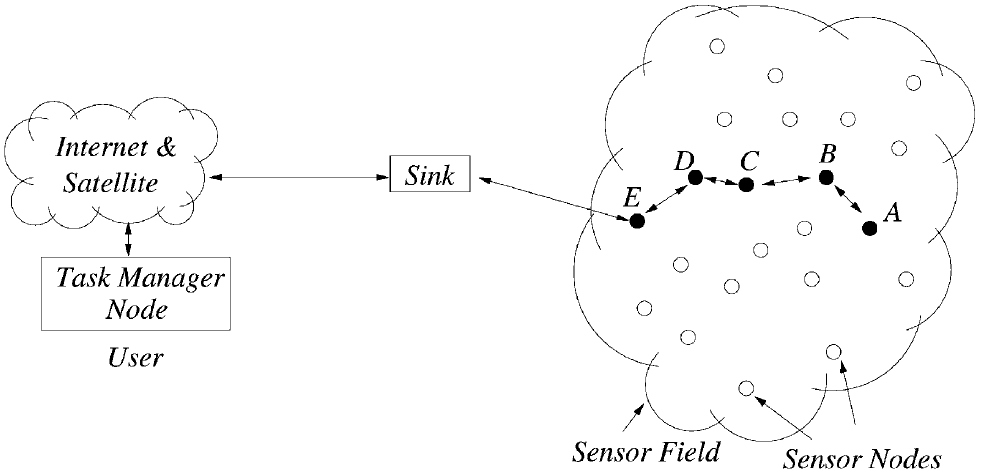
\includegraphics[scale=0.5]{Chapters/Figures/sensor_nodes_in_sensor_fields.png}
    \label{fig:sensor_nodes_in_sensor_fields}
\end{figure}

Typically, each node sensor is composed by a radio trasceiver, an embedded processor, internal
and external memories, a power source and one or more sensors \cite{Wang2010}. However, the
nodes' design and the WSN itself' must take into account its purpose, the environment where
the nodes will operate, the hardware, the cost, along with other restrictions that need to
be considered \cite{Yick2008}.


\subsection{Architecture}
\label{subsec:wsn_architecture}
The most common architecture for WSN follows the OSI model. This model is composed of five
layers: application layer, transport layer, network layer, data link layer and physical layer,
and three cross plane layers: power management plane, mobility management plane and task
management plane, as shown in Fig. \ref{fig:wsn_architecture}.

\begin{figure}[h]
    \caption{WSN Architecture \cite{Akyildiz2002}}
    \centering
    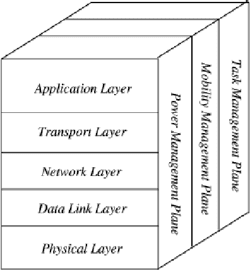
\includegraphics[scale=0.5]{Chapters/Figures/wsn_architecture.png}
    \label{fig:wsn_architecture}
\end{figure}

The five layers above mentioned work together to ensure the data is properly transmited to the
network, each with a specific functionality:
% TODO: layers explanation
\begin{description}
    \item[Application Layer]
    \item[Transport Layer]
    \item[Network Layer]
    \item[Data Link Layer]
    \item[Physical Layer]
\end{description}

The management planes' roles are to manage the network and optimize the sensor nodes'
performance in order to improve the overall effectiveness of the network, considering the
advantages acquired by all sensor nodes working together. Each of these planes manages
a specific area \cite{Akyildiz2002}:
\begin{description}
    \item[Power Management Plane] manages how the sensor node uses its power, chosing when to
        turn off its receiver to save energy or to keep it from receiving repeted messages. It
        also informes its neighbours when it reaches a low power mode.
    \item[Mobility Management Plane:] keeps track of the sensor nodes' neighbours and always
        disntinguishes a route back to the user.
    \item[Task Management Plane:] administers the periodicity and schedule that each node needs
        to maintain in order to perform their sensing tasks based on their power dependency and
        task requirements.
\end{description}

\subsection{Network Topologies}
There are several different topologies regarding the connection between nodes and their message
exchange routes \cite{Yadav2012, Lewis2004}:
\begin{description}
    \item[Star Topology:] all nodes are connected to only one node, the coordinator. This
        means every node will communicate via this central node and every node that requests
        to enter this network will have to send its information to the coordinator, which
        will then send it to the other nodes. The principal limitation of this topology is
        that if the coordinator malfunctions the whole network will fail.
    \item[Ring Topology:] all nodes are equal connected, having no coordinator. Contrarly
        to the star topology, if a single link is broken the whole network will fail.
    \item[Bus Topology:] all nodes broadcast their messages using the bus. Each message
        has a header with the destination address so that every node can see if the message
        is fot them or another node. This topology is passive, since the nodes are not
        responsible for retransmitting messages.
    \item[Tree Topology:] % TODO: find info
    \item[Fully Connected Topology:] every node is connected to every other node. This will
        lead to a routing problem when dealing with large networks.
    \item[Mesh Topology:] the nodes are generally identical, so the mesh connections are
        commonly referred as peer-to-peer connections. However, even though the nodes are
        generally identical some of them can be assign as coordinators that take additional
        functions and if one of these coordinators stops working, another just takes over his
        work. An interesting aspect of this topology is that the communicattion can be
        done between any two nodes in close proximity, which makes this topology quite
        robust to the failure of nodes or links and good for large scale networks.
\end{description}

\begin{figure}[h]
    \caption{Network Topologies \cite{Lewis2004}}
    \centering
    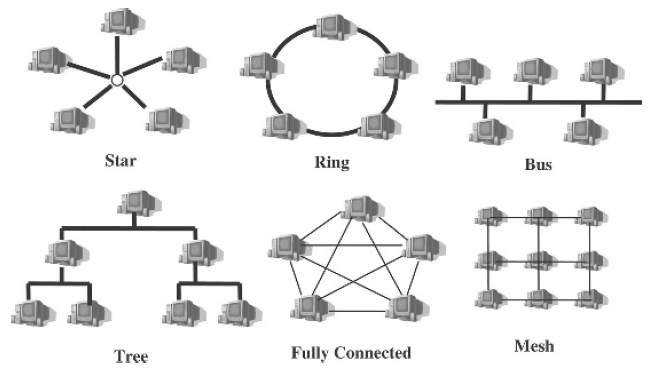
\includegraphics[scale=0.7]{Chapters/Figures/network_topologies.png}
    \label{fig:network_topologies}
\end{figure}

\subsection{Strategies}
\label{subsec:wsn_strategies}
The WSN have enumerous applications, this idea will be further discussed in the subsequent
subsection \ref{subsec:wsn_applications}, which will lead to different solutions for each of
them.

\subsection{Gossip in WSNs}
\label{subsec:gossip_in_wsns}
One of the main purposes of a sensor node is to transmite the data it has collected, via
the sensors, to the sink. The route chosen by these nodes is of the most importance,
therefore various protocols were studied in \cite{Akkaya2005} to understant which of
these would better conduct this task.

As presented previously in the section \ref{sec:gossip_protocol}, during the gossip protocol
each node only transmites its messages to \textit{t} randomly selected nodes and not the
whole network, as in the flooding protocol. This characteristic ensures that every node
in the gossip protocol will only have a single copy of the packet to be sent, which
adresses one of the shortcomings of the flooding protocol, the implosion. However, this
will lead to delays in the dissemination of the data which may be an important factor
for some applications of the network.

% Challenges of WSN: 
% Quality of Service
% Security Issue
% Energy Efficiency
% Network Throughput
% Performance
% Ability to cope with node failure
% Cross layer optimisation
% Scalability to large scale of deployment

\subsection{Applications}
\label{subsec:wsn_applications}
The applications of WSN is vaste, some of the areas are health, military, home, environmental
and many others.

%discussion -> most important is the low power

\subsubsection{ZebraNet}
\label{subsubsection:zebranet}

\subsubsection{Wireless Tracking}
\label{subsubsection:wireless_tracking}

%\section{Sensors and Arduino}
%\label{sec:sensors_and_arduino}

\section{Existing Collars}
\label{sec:existing_collars}

\section{Cows Habits}
\label{sec:cows}

\section{Summary}
\label{sec:summary}
